\begin{frame}{Les animaux de compagnie \gloss{Pets}}
  Quelle est la bonne conjugaison du verbe \lexi{avoir}? \\
  \tinygloss{What is the correct conjugation for the verb \lexi{avoir}?}
  \begin{columns}
    \column{0.6\textwidth}
      \begin{enumerate}
        \item Vous \underline{\uncover<2->{avez}} un chien.
        \item On \underline{\uncover<4->{\ a\ \ }} des poissons.
        \item J'\underline{\uncover<6->{\ ai\ }} des oiseaux.
        \item Elles \underline{\uncover<8->{ont\ }} un chat.
        \item M. McNeill \underline{\uncover<10->{\ a\ \ }} un lézard.
      \end{enumerate}
    \column{0.4\textwidth}
      \begin{minipage}[c][0.6\textheight]{\linewidth}
        \begin{center}
          \only<1-2>{
            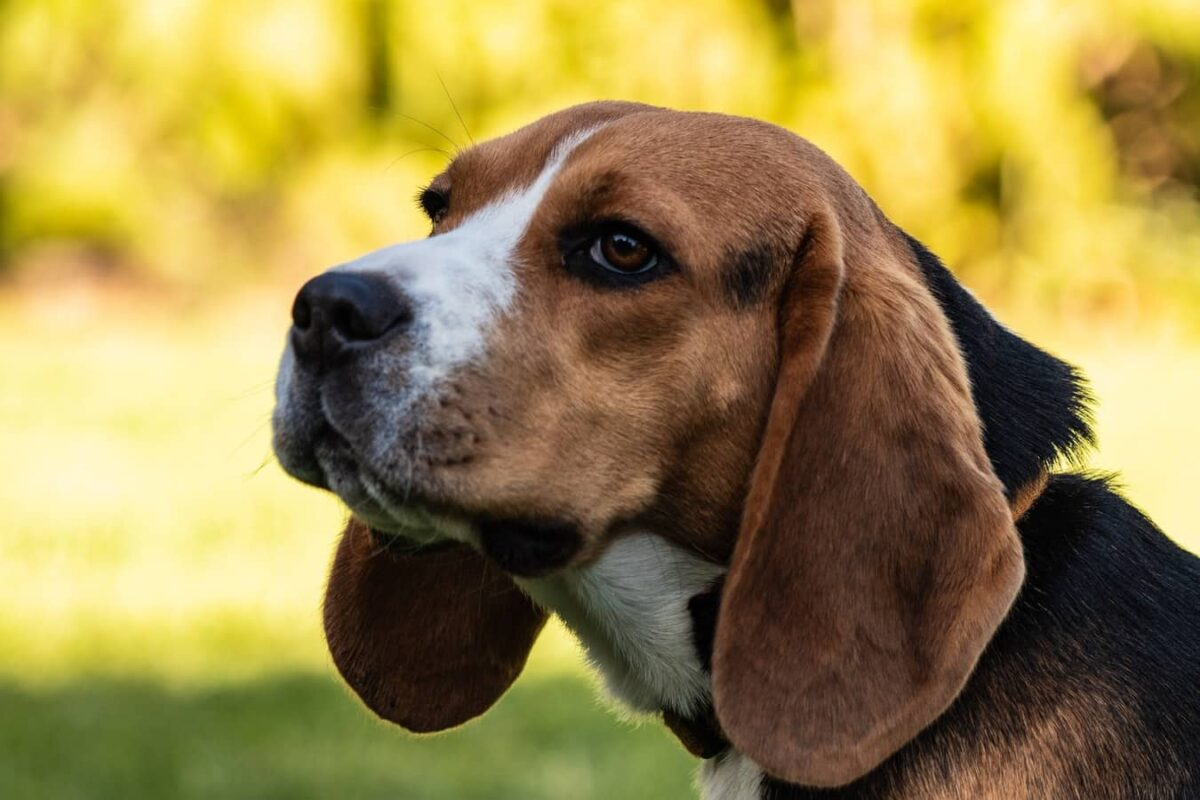
\includegraphics[scale=0.11]{chien.jpg}
          }
          \only<3-4>{
            
\includegraphics[scale=0.1]{aquaman.jpg}
          }
          \only<5-6>{
            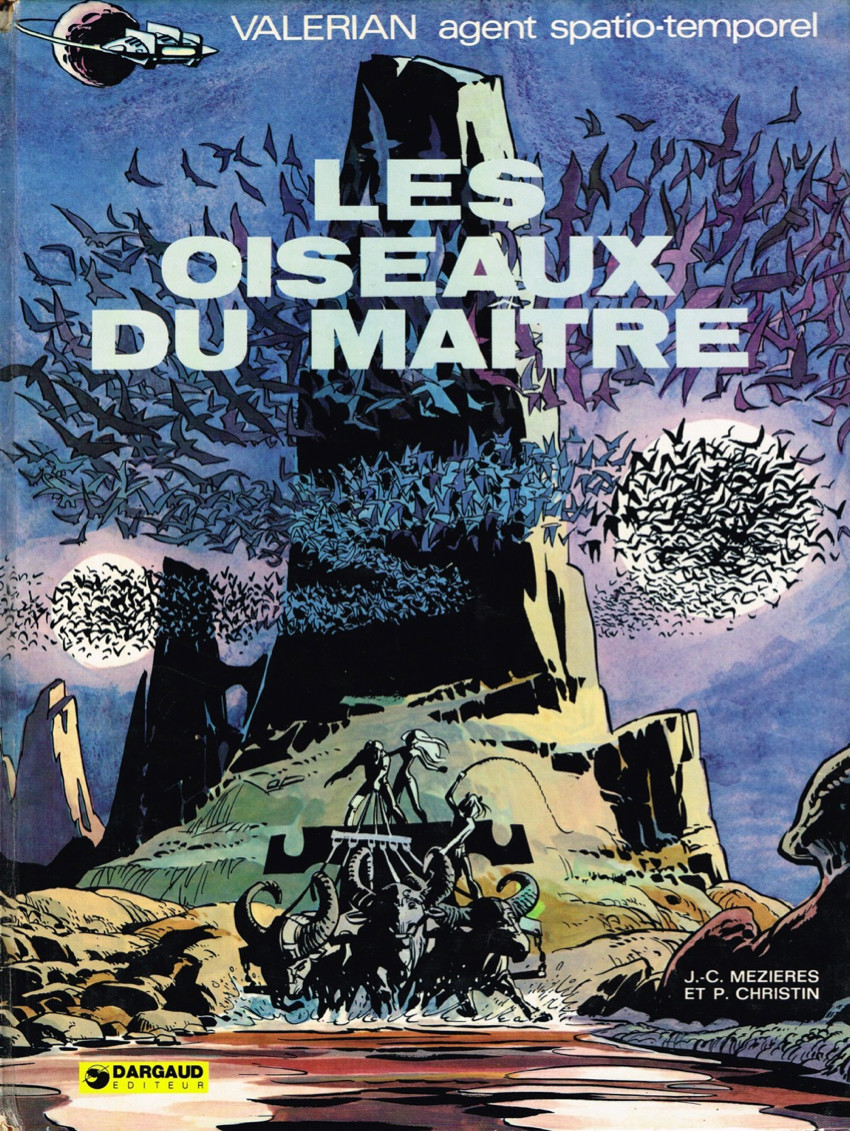
\includegraphics[scale=0.18]{oiseaux.jpg}
          }
          \only<7-8>{
            
\includegraphics[scale=0.5]{puss_in_boots.png}
          }
          \only<9-10>{
            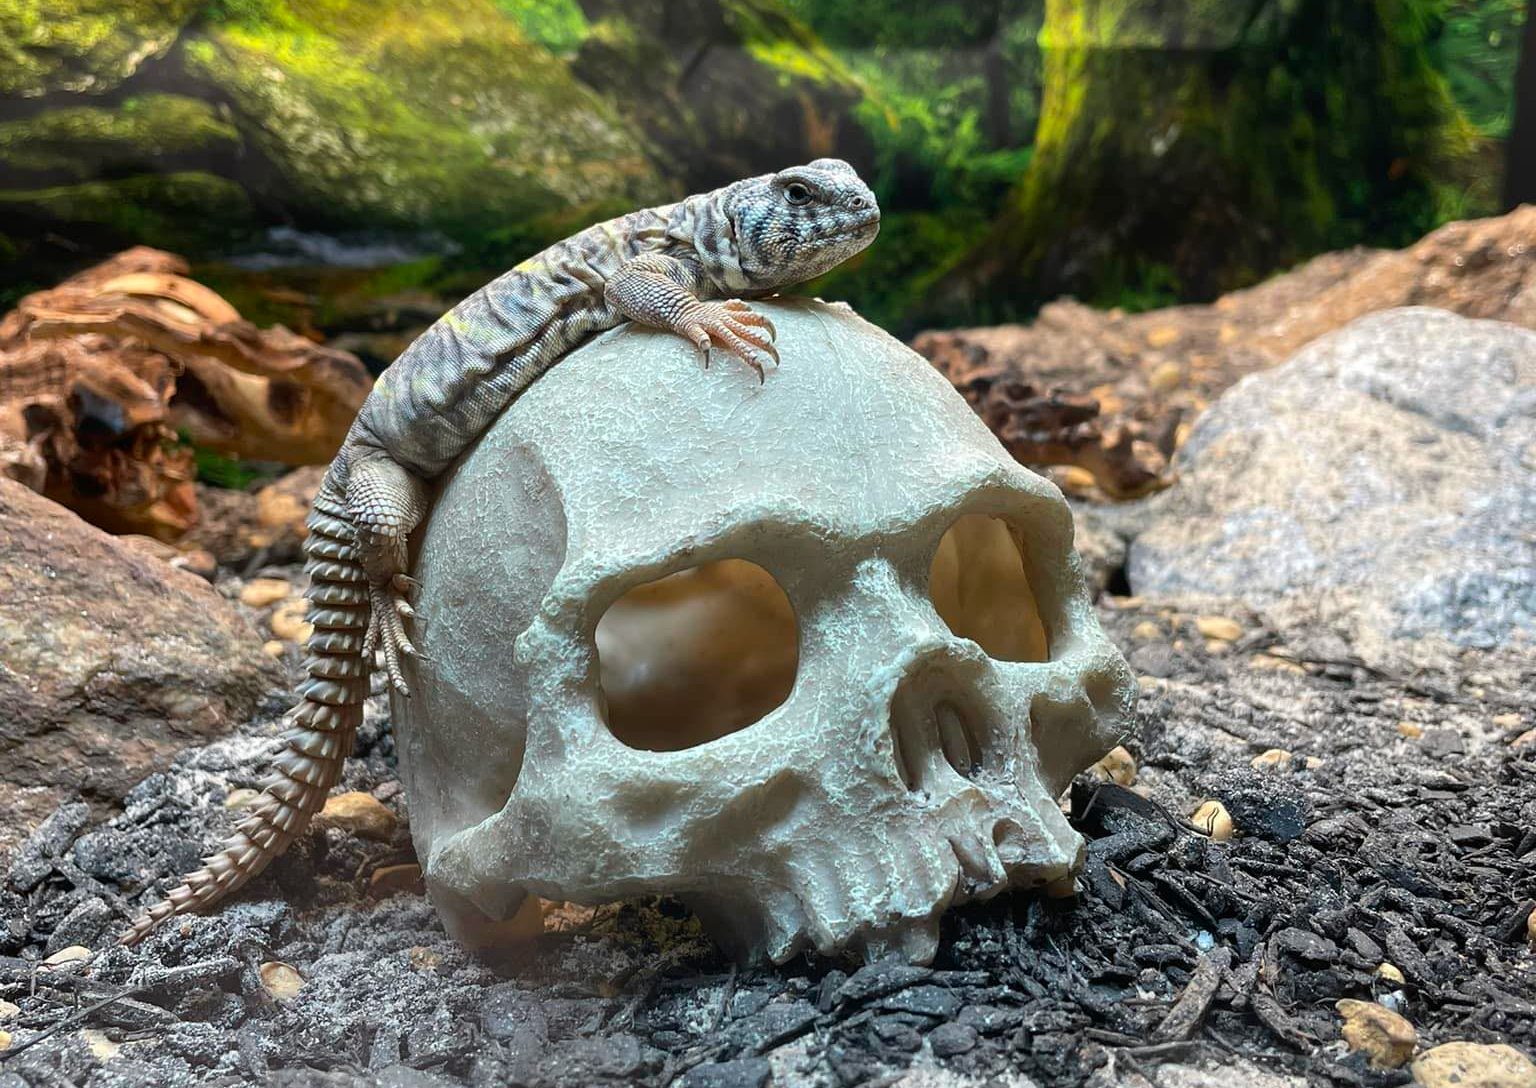
\includegraphics[scale=0.35]{milton.jpg}
          }
        \end{center}
      \end{minipage}
  \end{columns}
\end{frame}